\documentclass{article}

\usepackage[a4paper]{geometry}
\usepackage{amsmath,amssymb,amsthm}
\usepackage{times}
\usepackage{caption}
\usepackage{subcaption}
\usepackage{hyperref}
\usepackage{url}
\usepackage{mathtools}
\usepackage{graphicx}
\usepackage{algorithm,algorithmic}
\usepackage{natbib}
\begin{document}
\title{Large Scale Machine Learning - Assignment 4\\Abhishek Sinha, Arun Sai, Ashish Bora}
\maketitle
\section{Feature Extraction}
In this assignment we didn't focus much on data cleaning. We instead concentrated on feature extraction part. For data cleaning we relied on the public scripts that were posted on Kaggle. These scripts removed redundant columns and identified outliers and appropriately modified their feature values.
Below we describe some of the features we extracted. 
\subsection{Random Feature Combinations}
Here we generated new features by combining original features using arithmetic operators : $+, -, * , /$.
\begin{table}[h!]
\begin{center}
\begin{tabular}{ |c|c| } 
\hline
feature&AUC (Validation Set)\\ \hline
$pca4-ind\_var30$&0.7459055\\ \hline
$n0+var15$&0.7423217\\ \hline
$pca\_all0+num\_var13\_0$&0.7143601\\ \hline
$pca4+num\_op\_var39\_ult1$&0.7129791\\ \hline
$pca1+var15$&0.7128941\\ \hline
$ind\_var41\_0-pca2$&0.7096776\\ \hline
\end{tabular}
\end{center}
\caption{Table shows some of the important feature combinations found. Because of the huge number of possible combinations we randomly generated combinations and picked the top few and used them in training. The last column shows the AUC obtained on the validation set by fitting a decision tree($depth=3$) using the feature on the left column. Features Names: $pca*$ denotes features obtained through PCA on the original dataset and $n0$  represents number of zeros.}
\end{table}
\subsection{Random Rotation of Feature Space}
This is related to the question we posted on piazza about training better decision trees by finding a rotated feature space on which decision trees can generalize better. We couldn't come up with a principled \& efficient approach to do this. So we randomly rotated the feature space and trained a model using XGB on the rotated space. However random rotations didn't work well (AUC approximately dropped by $10\%$). 
\subsection{KNN}
This feature is based on the KNN classifier. Here we first built a kd-tree on the combined dataset of train and test sets. We then
extracted features such as : number of positive labels that are close to a given point. This feature resulted in over fitting (the public LB score is significantly lower than the CV score obtained when this feature was used in training).
\subsection{Other Features}
\begin{itemize}
\item \textit{PCA:} Extracted the top 10 principal components using the entire training data and using only the important features.
\item \textit{KMeans:} Here we clustered the training and test datasets and added the resulting cluster id of each point as a feature.
\end{itemize}
\section{Training}
We trained the following models: XGB, Random Forests, Extremely Random Trees, LR, Neural Nets. Needless to say, XGB performed the best out of these classifiers. To reduce the training time, we trained most of our models with $\sim$50 features that are important. This didn't significantly change the public LB score.
\subsection{XGB}
\begin{figure*}[tbh]
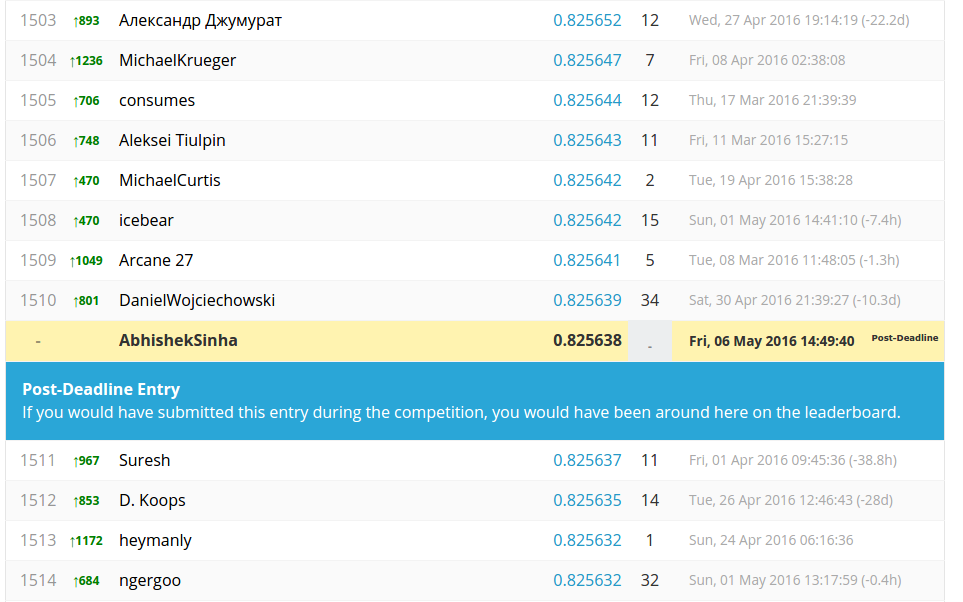
\includegraphics[scale = 0.4]{xgb}
\caption{XGB}
\label{4a}
\end{figure*}

\subsection{Logistic Regression}
We tried logisitc regression with L1 and L2 regularization. The C parameter was selected by standard 5-fold cross validation with logarithmic sampling and roc-auc metric. The score with L1 regularization was considerably better (0.7924) as compared to L2 regularization (0.615). The dataset is very sparse. Since L1 encourages sparse weight vectors, it probably does a better job of finding good features from a very sparse dataset.

\subsection{Neural Nets}
We used the Keras script given in the forums. This uses 3 fully connected layers from 81 to 400, 400 to 200 and finally 200 to 1. It uses \emph{tanh} non-linearities. There is also a sigmoid at the end and the loss used is again binary cross entropy.  The whole network is trained with the Adam Optimizer. It seems that the author faced problems of skewed data. To address this, they just end up using only around 6000 training examples (3000 each of positive and negative) so as to make their dataset balanced. Despite getting rid of so much data, this network achieved a public Kaggle score of $0.789466$.
\begin{figure*}[tbh]
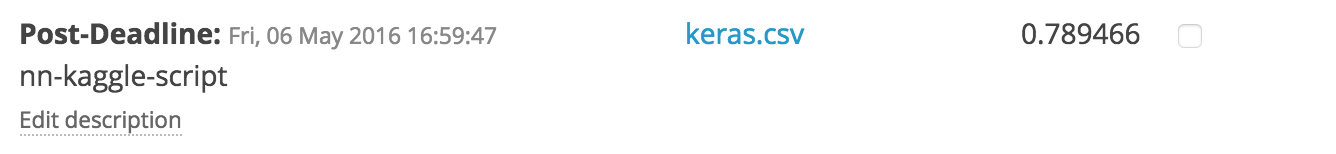
\includegraphics[scale = 0.7]{nn2}
\caption{Neural Network}
\end{figure*}
\section{Ensemble}
We experimented with various ensembling techniques for this assignment. We ensembled all the classifiers described in the previous section. Here are different approaches we tried:
\begin{itemize}
\item \textit{Weighted average:} average based on the CV score.
\item \textit{Rank averaging:} weighted average after converting to ranks.
\item \textit{Blending:} Here we trained a meta model which takes the predictions from all the base classifiers and learns to combine their predictions. We experimented with various meta models: LR, RF, XGB.
\end{itemize}
While blending (with XGB/RF as meta models) performed better than simple averaging, it didn't significantly outperform the best XGB model (\textit{i.e,} we didn't see much gains using blending). 

\end{document}